\documentclass[a4paper]{jpconf}
\usepackage{graphicx}
\usepackage{booktabs}
\usepackage{siunitx}
\usepackage{enumitem}
\usepackage[options]{biblatex}

\usepackage{subfig,multicol}
\usepackage[export]{adjustbox}
\usepackage{float}


\usepackage[utf8]{inputenc}
\usepackage[english]{babel}
\usepackage{fancyhdr}
\usepackage{lastpage}

\pagestyle{fancy}
\fancyhf{}


\rfoot{Page \thepage \hspace{1pt} of \pageref{LastPage}}


\addbibresource{Congested.bib}
\nocite{*}



\begin{document}
\title{Towards a city congestion index: methodological explorations using Google's Distance Matrix API}

\author{Jonathan Cohen and Jorge Gil}

\address{Chalmers University of Technology, Sven Hultins gata 6, SE-412 96, Göteborg, Sweden}

\ead{jonathan.cohen@chalmers.se}




\begin{abstract}
	All articles {\it must} contain an abstract. This document describes the  preparation of a conference paper to be published in \jpcs\ using \LaTeXe\ and the \cls\ class file. The abstract text should be formatted using 10 point font and indented 25 mm from the left margin. Leave 10 mm space after the abstract before you begin the main text of your article. The text of your article should start on the same page as the abstract. The abstract follows the addresses and should give readers concise information about the content of the article and indicate the main results obtained and conclusions drawn. As the abstract is not part of the text it should be complete in itself; no table numbers, figure numbers, references or displayed mathematical expressions should be included. It should be suitable for direct inclusion in abstracting services and should not normally exceed 200 words. The abstract should generally be restricted to a single paragraph. Since contemporary information-retrieval systems rely heavily on the content of titles and abstracts to identify relevant articles in literature searches, great care should be taken in constructing both.
\end{abstract}

\

\section{Introduction}
\indent What are the problems with congestion? Is it mentioned in UN Habitat NUA, or SDGs e.g.11?\par
the goals of dealing with congestion (especially in the SDG). the negative consequences of congestion on the environment and people. Use some references.
\indent What are the clients of this index? Who needs such an index, and to do what?\par
The importance of planning to avoid congestion, how transport plannign focuses on flows and capacity of the infrastructure, but given what we know on iduced demand (ref) this is not always a viable solution. the need for spatial planning, therefore for a spatial understanding of the problem to mitigate.

\section{Theoretical background}
how is congestion defined. by one or two authors only.
The components of congestion: the route between OD pair, the distance and travel time (consequently, the speed of travel), the capacity of the route. inherently a travel time difference problem.
The components of a broader understanding of the phenomenon: a person travelling with a purpose, a date and time of day, two locations (origin and destination). This brings it closer to definitions of accessibility, but measuring the convenience of travel (refs on this?)
\indent What congestion indices exist out there? \par
How it is measured (absolute and relative indices)
\indent Practice/literature\par


\indent How are others mapping congestion (or real travel time) with geodata? (edited) \par
The focus on the link (flow and speed), the focus on visualisation.





\indent As the list of traffic congestion indicators
As the list of 
At the same time new methodologies to measure traffic congestion were developed, researchers 


At the same time different 

some researcher were 

For instance in Lomax (1993) 

In parallel, as the list of traffic congestion measurements increased 








\section{Research Aim}
\indent As mentioned above, traffic congestion is an urban problem that deteriorate the positive benefits of urban life, therefore is imperative to understand the problem in depth and look at it from different angles. Traditional congestion measurements are found to be costly and through practice or research different methods have been explored to overcome this issue. \par
\indent One avenue of research understands congestion as a time and location specific problem, which occurs in a road segment and that its consequences are suffered from those in the immediate surroundings. A second understanding of the problem deals with the individuals who are affected by traffic. \par
\indent Focusing on this second interpretation of the problem, the aim of this research is to provide a methodology to spatialize congestion to expose how traffic congestion is distributed across an urban area. The map of congestion can provide useful information to local authorities and planners since more disaggregated spatial information will be provided. \par



\section{Methodology}
\indent At its core the methodology described in this section details a process of collecting and processing data from an internet service that provides traffic estimations and routing optimization. The method presented here correspond to data extracted from the Distance Matrix API form Google Inc., but the exact same exercise could be done with other services such as HERE or TOMTOM.\par
\indent Given the quantity and nature the methodology that will be described above, was coded and executed using R in Rstudio and the functions written can be found in GitHub. \par
\indent In order to prioritize clarity over narrative, the necessary steps followed by this methodology are listed below: 
\begin{enumerate}[label=\arabic*)]
	\item Select and define an urban area to work with: After an urban area is selected a synthetic boundary needs to be drawn. In this case, for simplicity reasons, a circular buffer zone was used to define the 'study area'.
	\item Choose a zoned cartography of the area and clip it accordingly to the boundaries: Choose from any geographical authority a zoned cartography. Census tracks, neighbourhoods or plots can be chosen. In our case the European Population grids was selected.	
	\item Make centroids from the zones and extract the geographical position of each point
	\item Generate permutations from centroids to create an empty Origin-Destiny Matrix: Using the GPS location (latitude and longitude) of each centroid, a list of all possible combinations is generated (a total of n*(n-1) routes).  For instance, is the area to be studied contains 3 areas (A, B \& C), the OD matrix will consider the following routes: (i) A to B, (ii) A to C, (iii) B to A, (iv) B to C, (v) C to A \& (vi) C to B. 
	\item Define a \textit{congested} and \textit{non-congested} times: Using the difference between a \textit{congested} and \textit{non-congested} situation as the definition of congestion, a time need to be specified. As information from Google will be used, a future time needs to be specified. Based on previous results, Thursday, October 15, 2020 8:30:00 AM was chosen as a \textit{congested} moment and Wednesday, July 15, 2020 3:30:00 AM, as a \textit{non-congested}.
	\item Use a routing service to estimate time and distance travelled: The origin to destination list with the \textit{congested} and \textit{non-congested} time specification were used as inputs for the routing service to estimate travel time and distance. 
	\item Calculate descriptive statistics and visualize: Histograms, scatter plots and descriptive statistics were calculated to detect possible  problems such as missing data or outliers. 
	\item Deal with data issues: As the centroid of the polygon based on the European Population Grid could fall over a problematic place such as river, park or railway lot (places where google maps cannot match an address), some routes could not be retrieved and consequently were left out of the study.
	\item Calculate KPIs: Based on research done in the past the following can be derived:
		\begin{itemize}
			\item Time difference:			
			\item Relative time difference:
			\item Average travel speed:
			\item Average travel speed difference:
			\item Relative travel speed difference:
			\item Travel Time Index (TTI):			
		\end{itemize}	
	\item Aggregate data generated and join to spatial grid: With the data retrieved averages by the origins were calculated and joined to these values joined to the original zoned urban area. 
	\item Calculate descriptive statistics and visualize: The results at the Grid level are analyzed using descriptive statitics and basic plotting. This step can be seen as check-up point that can contribute to identify data anomalies such as missing data or outliers. 
	\item Map the results: Finally, once the data clean-up process is done, a map with the processed variables can be generated.
\end{enumerate}

\indent To demostrate how the method could be used in practice, four European cities where selected as a proof of concept.\par


\section{Data}
\indent In order to run the analysis for a desired urban area, a zoned cartography of the area is needed. In this opportunity, as a proof of concept the 1km2 population grid from the EuroStat (GEOSTAT 2011) was used. Amsterdam, Glasgow, Goteborg and Lisbon were selected and from their historical centre a buffer zone was used to delimit the \textit{city} boundary. The geographic coordinates of the centroid of each 1km2 square was used to create the list of all possible routes. \par
\indent The list of all possible origins to all possible destinations was then used to retrieve data for a \textit{congested} and \textit{non-congested} moments. 

\subsection{Data retrieved}
The process generates information for a total n*(n-1) routes (n being the number of zones). For instance, Lisbon is divided into 119 squares and the number of possible routes is 119*118 = 14,042 (then 28,084 travels were estimated). Amsterdam has 131 zones, Glasgow 136 and Goteborg 123 (17,030, 18,360 and 15,006 routes respectively). A summary of the descriptive statistics for the time in minutes can be found in Table \ref{tab:Results_routes}.

\begin{table}[ht]		
	\centering
	\begin{tabular}{rlrrrrr}
		\hline
		& Congested scenario (mins) & Routes & Mean & S.D. & Min & Max 	   \\ 
		\hline
		1 & Amsterdam 	& 17,023 & 20.26 & 6.86 	& 0.65 & 48.57 		   \\ 
		2 & Glasgow 	& 18,355 & 23.08 & 8.68 	& 1.42 & 56.88 		   \\ 
		3 & Goteborg 	& 14,997 & 18.01 & 6.82 	& 1.37 & 57.97 	       \\ 
		4 & Lisbon 		& 14,043 & 28.16 & 11.70 	& 1.37 & 84.63 	       \\ 
		
		\hline
		& Non-Congested scenario & Routes & Mean & S.D. & Min & Max    \\ 
		\hline
		1 & Amsterdam	& 17,023 & 11.70 & 3.71 & 0.52 & 24.90 	       \\ 
		2 & Glasgow 	& 18,355 & 11.93 & 3.99 & 0.83 & 24.85 	       \\ 
		3 & Goteborg 	& 14,997 & 13.09 & 5.29 & 1.10 & 49.18 	       \\ 
		4 & Lisbon 		& 14,043 & 12.82 & 5.77 & 0.77 & 46.90         \\ 
		\hline
	\end{tabular}
	\caption {Descriptive Statistics of travel times by city}
	\label{tab:Results_routes}
\end{table}

\indent The amount of route information retrieved is consistent with the amount of zones in the city and as expected, the \textit{congested} situation on average takes longer time. Formally an independent-samples t-test was conducted to compare the travel times under a \textit{congested} and \textit{non-congested} situations. For each city, the time difference was found statistically significant with a confidence level of 99\%.


\section{Results}
After capturing, processing and aggregating the data obtained from the API, table \ref{tab:Results_grids} on page ~\pageref{tab:Results_grids} contains the descriptive statistics for time difference and TTI. In this case, the number of observations corresponds to the number of zones in the map and each zone holds the mean of all the trips departed from that origin. 
\indent The results show that the methodology successfully captured diversity between cities. For instance, in Lisbon the average time difference is of 15.3 mins, with a maximum of 21.6 mins, meanwhile in Goteborg on average delays are of 4.9 mins with a maximum of 8 mins.  

\begin{table}[ht]		
	\centering
	\begin{tabular}{rlrrrrr}
		\hline
		  & Time Difference (mins) & Zones & Mean & S.D. & Min & Max \\ 
		\hline
		1 & Amsterdam 	& 131 	& 8.57  & 2.39 & 5.38 & 19.03 \\ 
		2 & Glasgow 	& 136 	& 11.15 & 1.88 & 7.66 & 15.64 \\ 
		3 & Goteborg 	& 123 	& 4.92  & 0.99 & 3.22 & 8.06  \\ 
		4 & Lisbon 		& 119 	& 15.34 & 2.67 & 9.74 & 21.57 \\ 
		
		\hline
		  & TTI	& Zones & Mean & S.D. & Min & Max \\ 
		\hline
		1 & Amsterdam 	& 131 & 1.74 & 0.23 & 1.36 & 2.61 \\ 
		2 & Glasgow 	& 136 & 1.94 & 0.14 & 1.60 & 2.31 \\ 
		3 & Goteborg	& 123 & 1.38 & 0.09 & 1.21 & 1.69 \\ 
		4 & Lisbon 		& 119 & 2.21 & 0.16 & 1.70 & 2.57 \\ 
		\hline
	\end{tabular}
	\caption {Aggregated descriptive statistics by zones}
	\label{tab:Results_grids}
\end{table}

\indent Although, the table above reveals relevant insights about these cities, local authorities or planners would not know which places or who is being affected by traffic congestion. Therefore, in figure \ref{fig:result_tti} the TTI for each city was mapped. By looking at these maps several conclusions about where and how bad congestion is across the city. For instance, in all four cities, although the historical centre is the nearest point to all other destinations, when congestion is taken into account, these places face the highest TTI. This indicates that in a \textit{non-congested} situation, the city centre is highly accessible but when \textit{congested}, the advantage of being central gets eroded. \par
\indent These maps also show that the methodology presented in this study 
was able to capture differences across cities successfully. In Goteborg, the historical city centre gets mainly congested, meanwhile the other parts of the city remain with similar levels of congestion. In Lisbon, traffic congestion is more scattered accross the city, presenting islands of low congestion (where the CBD and commercial areas have moved to).


\begin{figure}[H]
	\centering
	\begin{multicols}{2}
		\noindent
		%
		\subfloat[Amsterdam]{\centering
			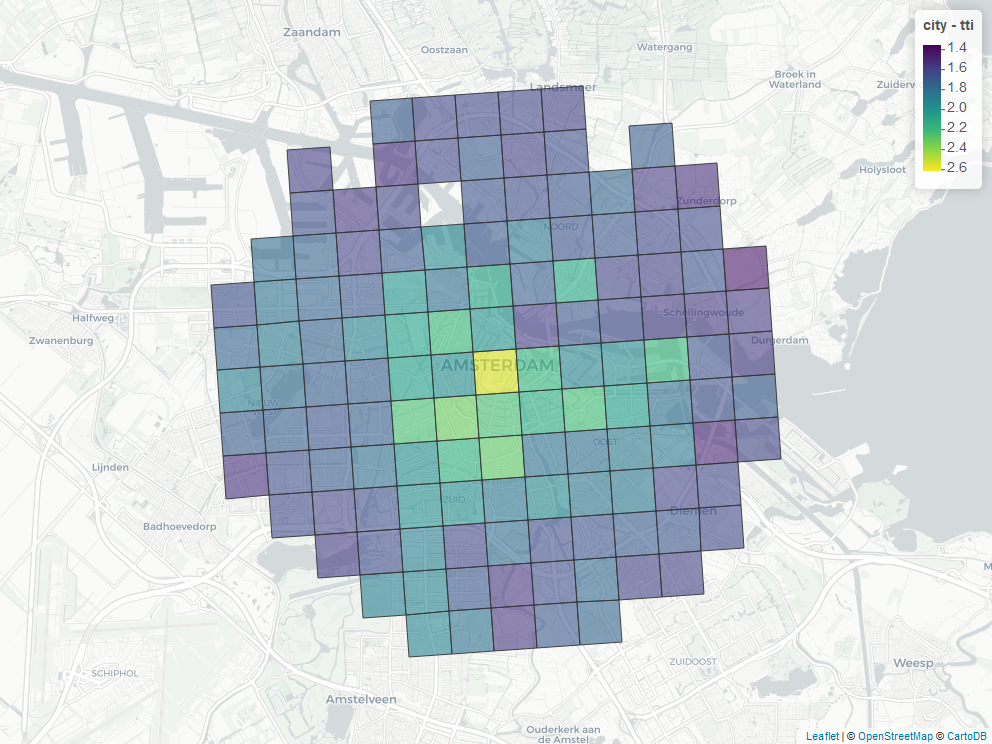
\includegraphics[width=0.8\linewidth, height=4cm]{./Img/amsterdam_tti}} \par 
		%
		\subfloat[Glasgow]{\centering
			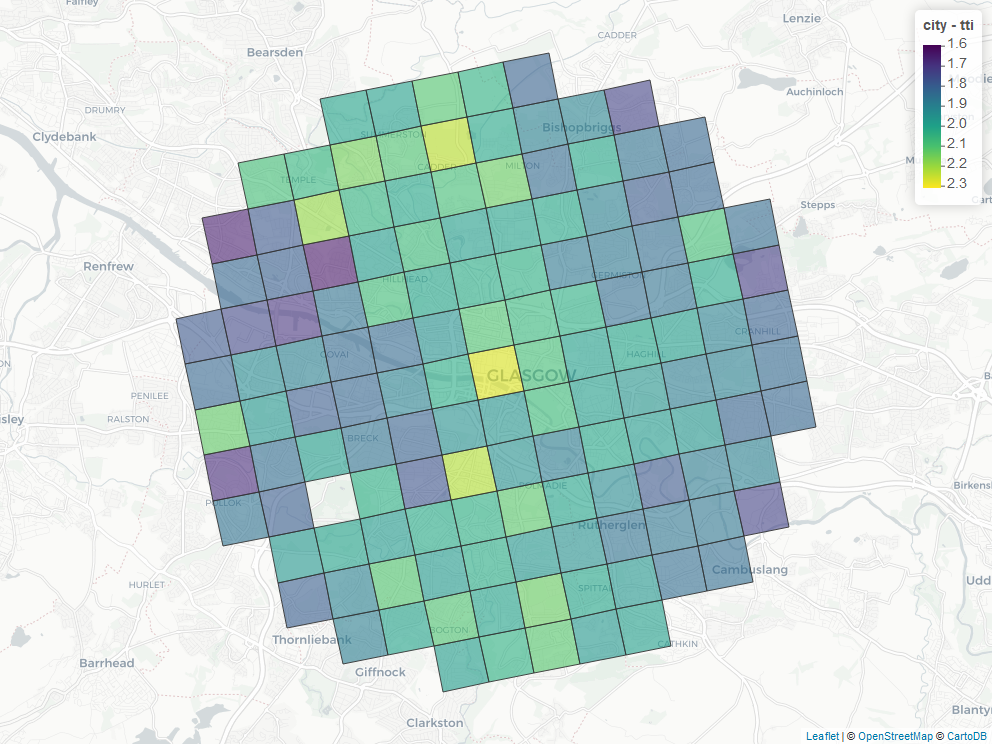
\includegraphics[width=0.8\linewidth,height=4cm]{./Img/glasgow_tti}} \newpage
		%
		\subfloat[Goteborg]{\centering
			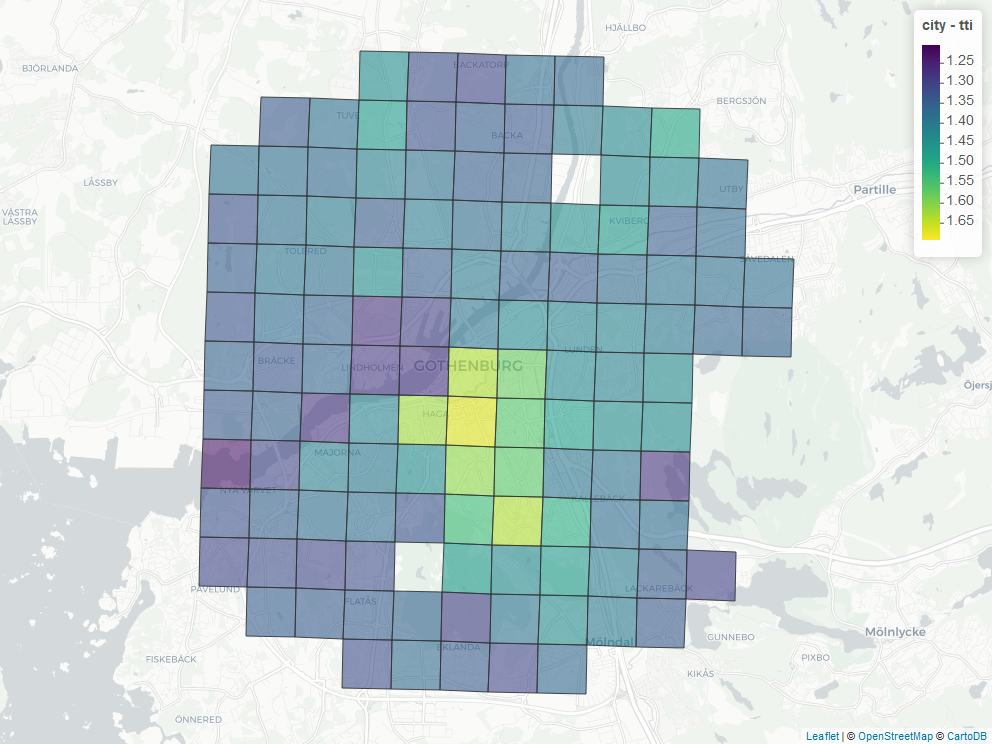
\includegraphics[width=0.8\linewidth,height=4cm]{./Img/goteborg_tti}} \par
		%
		\subfloat[Lisbon]{\centering
			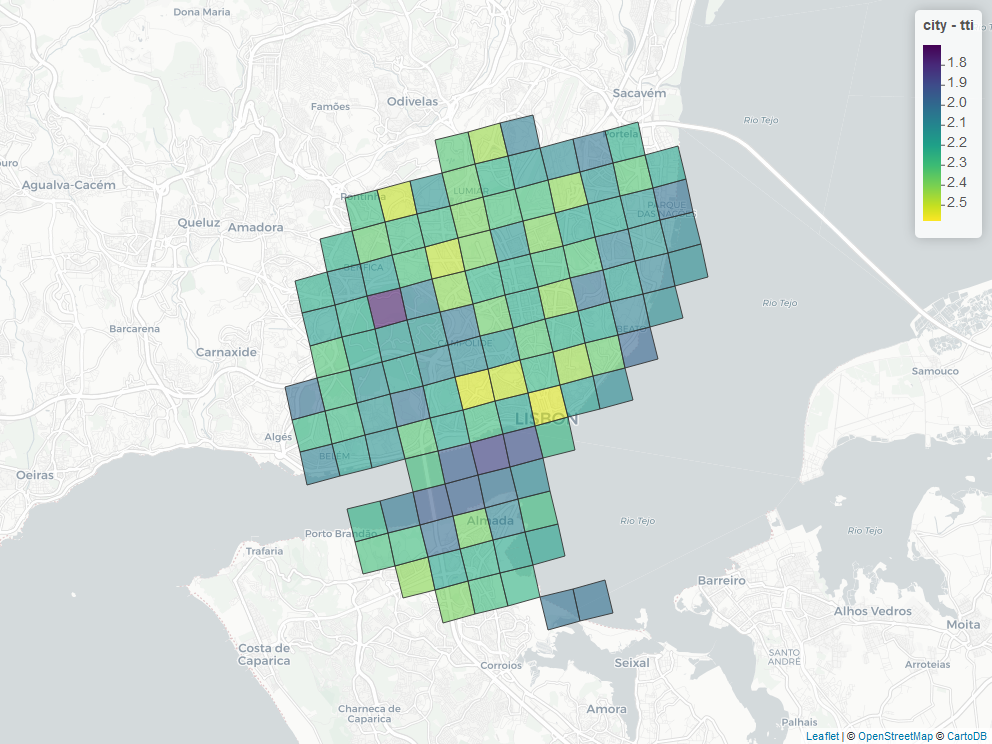
\includegraphics[width=0.8\linewidth, height=4cm]{./Img/lisbon_tti}} \par
		%	
	\end{multicols}
	\caption{Images extracted from results}
	\label{fig:result_tti}
\end{figure}


\begin{figure}[H]
	\centering
	\begin{multicols}{2}
		\noindent
		%
		\subfloat[Amsterdam]{\centering
			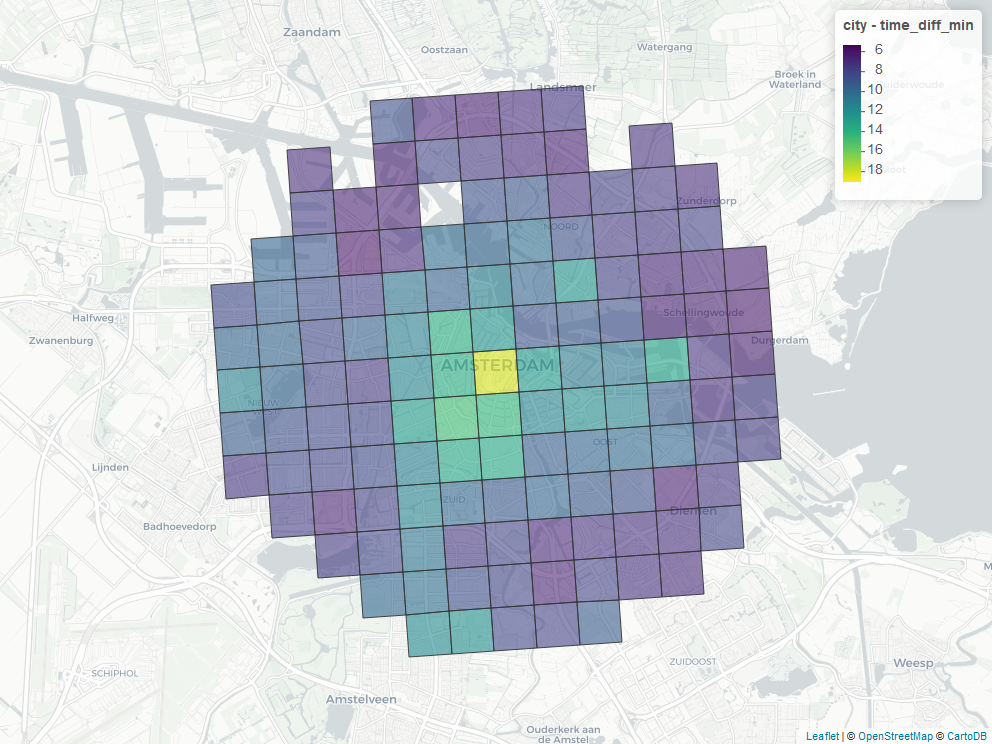
\includegraphics[width=0.8\linewidth, height=4cm]{./Img/amsterdam_time_diff_min}} \par 
		%
		\subfloat[Glasgow]{\centering
			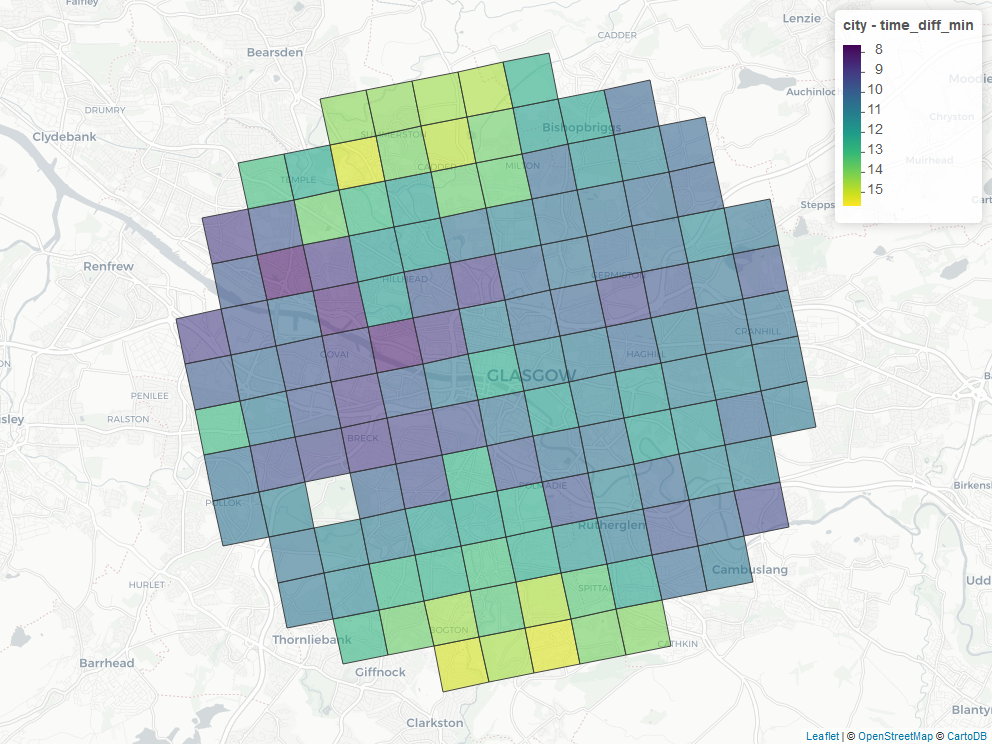
\includegraphics[width=0.8\linewidth,height=4cm]{./Img/glasgow_time_diff_min}} \newpage
		%
		\subfloat[Goteborg]{\centering
			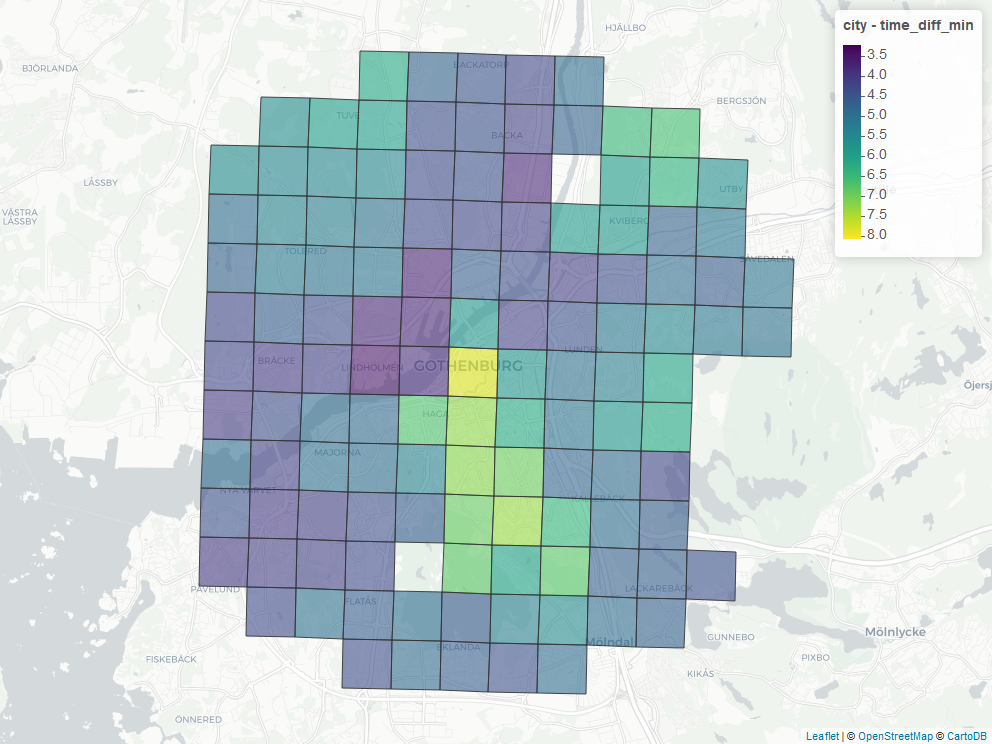
\includegraphics[width=0.8\linewidth,height=4cm]{./Img/goteborg_time_diff_min}} \par
		%
		\subfloat[Lisbon]{\centering
			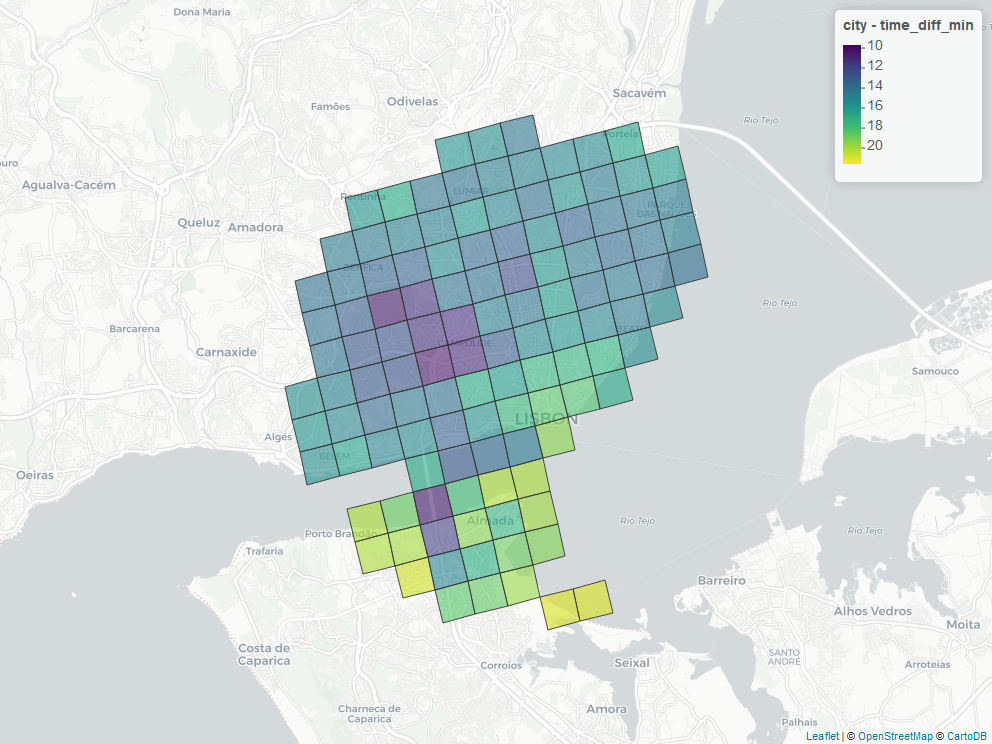
\includegraphics[width=0.8\linewidth, height=4cm]{./Img/lisbon_time_diff_min}} \par
		%	
	\end{multicols}
	\caption{Images extracted from results}
	\label{fig:result_diff}
\end{figure}



\section{Discussion}
\indent The methodology presented in this paper exploits a new data source to provide spatial insights about traffic congestion in different cities. The information generated allows planning and transport agencies to reconstruct some of the most popular indexes discussed in the literature review. \par 
\indent After aggregating the data retrieved from the Google API at the city level, the results were found to be consistent with the conclusion drawn by INRIX and TomTom.\par

\subsection{Grid size and shape}
\indent 

\subsection{Scalability}
address the generality of the method with global coverage
granularity (the choice of grid size? or the use of different spatial entities like census track or travel zones)
area covered

can use other APIs, like here, waze, tomtom
processing time. give rough examples

\subsection{Limitations and future work}
\indent Costs of operation of the method.
give details of the specific ones
will vary with the granularity and the coverage
will vary with the data source


\subsection{Applications}
\indent As shown \cite{Lomax1997} Traffic congestion measurements can be used  


\subsection{Limitations and future work}
\indent Grid size and costs
In this case 


\indent Weights
using population
using an OD matrix

1km grid size can be too coarse for spatial planning, has impact o

\indent use census tracks or population statistics to correlate with socio-demographics

\indent use census tracks or population statistics to correlate with socio-demographics 

\indent Reviewer Remarks:This is a very interesting paper proposal. It will be interesting to learn how the impact of different types of car engines (petrol, diesel, electric, etc) will impact CO2 emissions in congested and non-congested traffic flows.


\section{Conclusion}





%\section*{References}






\printbibliography





\end{document}






%
%
%\begin{figure}[H]
%	\centering	
%	\begin{multicols}{4}
%		\noindent
%		\subfloat[Data Science]{\centering
%			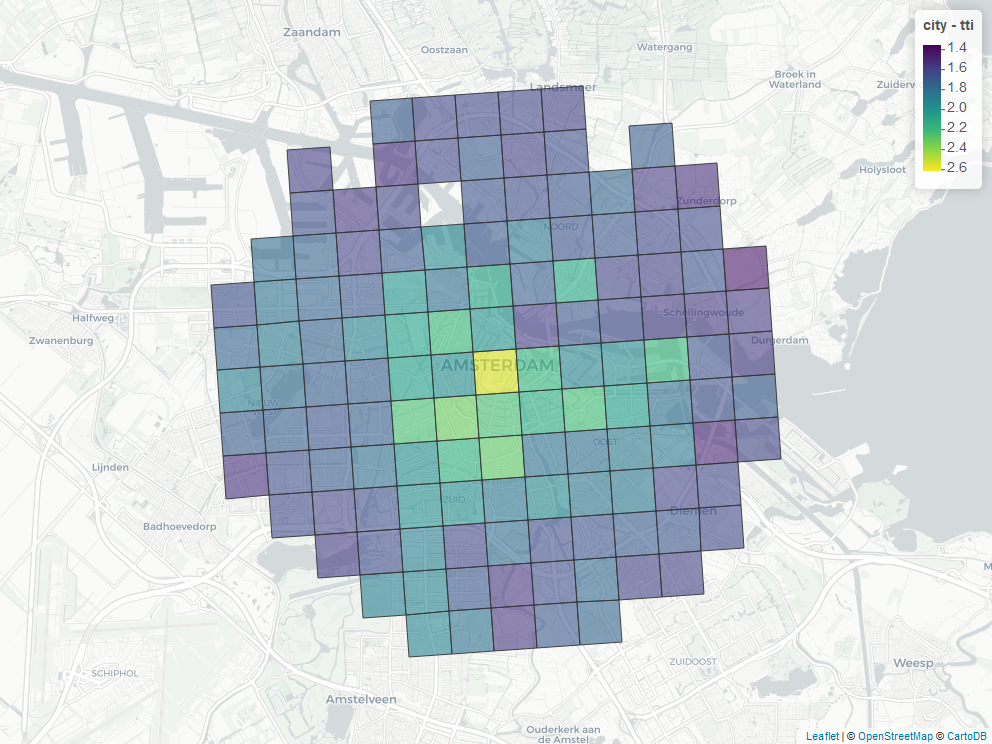
\includegraphics[width=1\linewidth, height=5cm]{./Img/amsterdam_tti}} \par 
%		%
%		\subfloat[New Data Sources]{\centering
%			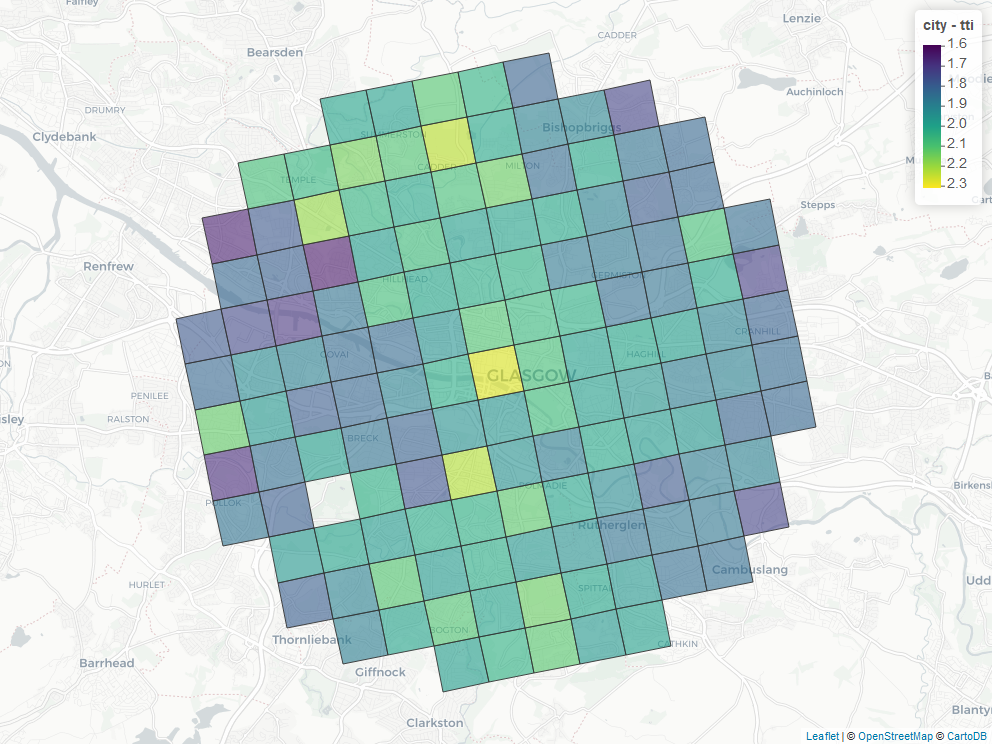
\includegraphics[width=1\linewidth,height=5cm]{./Img/glasgow_tti}} \par
%		%
%		\subfloat[Data Capture]{\centering
%			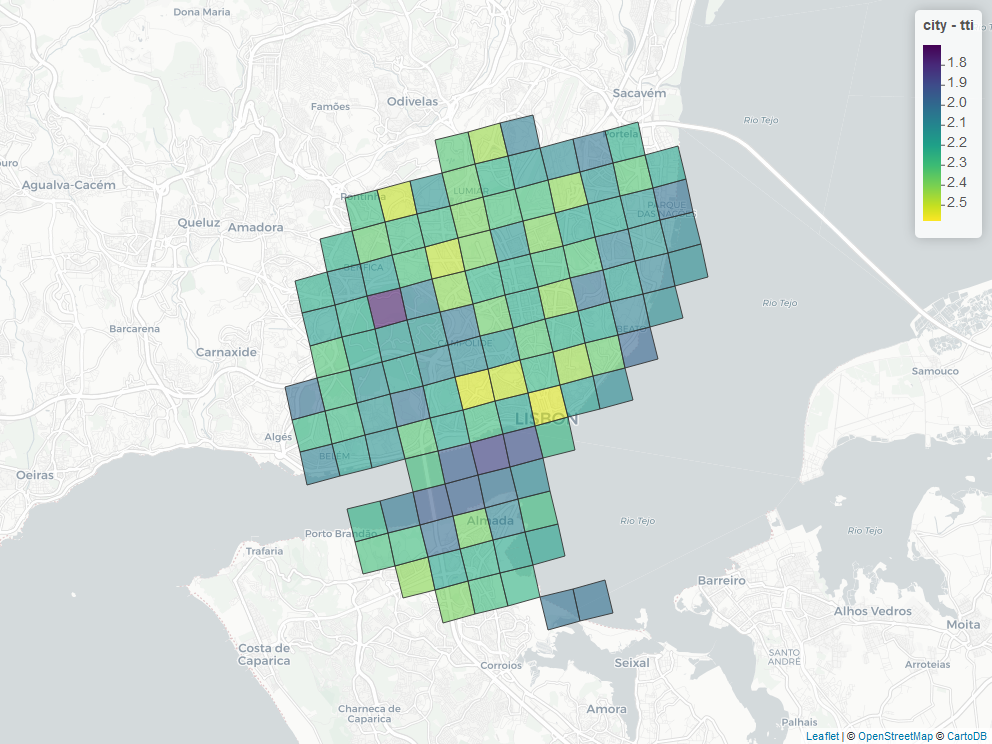
\includegraphics[width=1\linewidth,height=5cm]{./Img/lisbon_tti}} \par
%		%
%		\subfloat[Visualization]{\centering
%			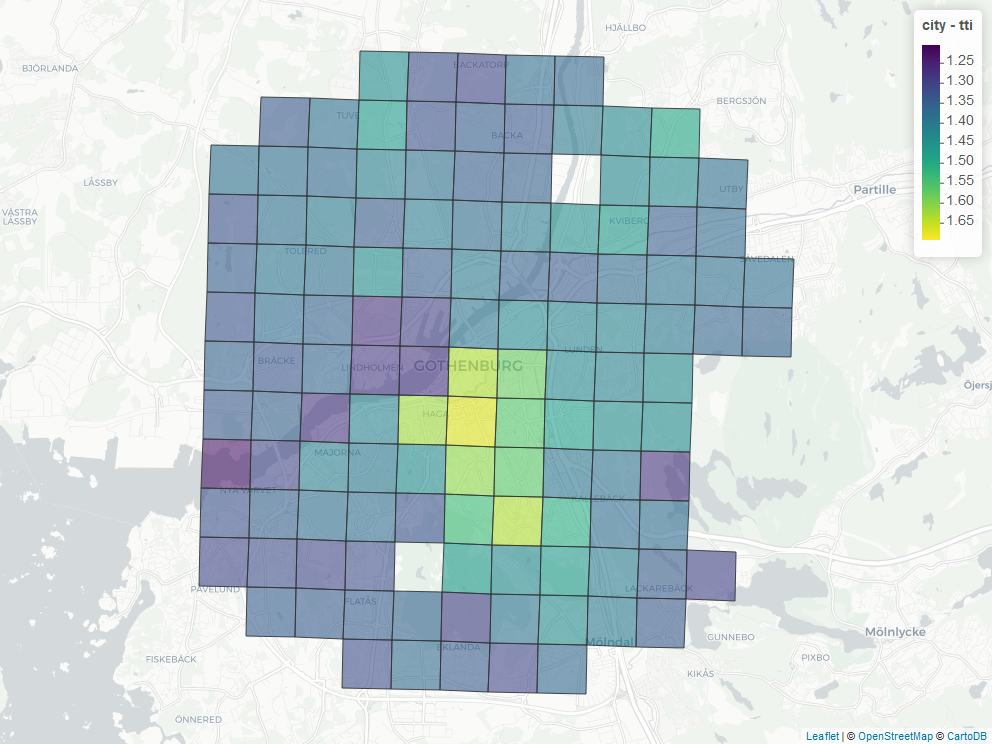
\includegraphics[width=1\linewidth, height=5cm]{./Img/goteborg_tti}} \newpage
%		%
%		\subfloat[Data Capture]{\centering
%			\includegraphics[width=1\linewidth,height=4cm]{./Img/2_1.PNG}} \par
%		%
%		\subfloat[Visualization]{\centering
%			\includegraphics[width=1\linewidth, height=4cm]{./Img/2_2.PNG}} \par
%		%
%		\subfloat[Data Capture]{\centering
%			\includegraphics[width=1\linewidth,height=4cm]{./Img/2_3.PNG}} \par
%		%
%		\subfloat[Visualization]{\centering
%			\includegraphics[width=1\linewidth, height=4cm]{./Img/2_4.PNG}} \newpage
%		%
%		\subfloat[Visualization]{\centering
%			\includegraphics[width=1\linewidth, height=4cm]{./Img/3_1.PNG}} \par
%		%
%		\subfloat[Data Capture]{\centering
%			\includegraphics[width=1\linewidth,height=4cm]{./Img/3_2.PNG}} \par
%		%
%		\subfloat[Data Capture]{\centering
%			\includegraphics[width=1\linewidth,height=4cm]{./Img/3_3.PNG}} \par
%		%
%		\subfloat[Visualization]{\centering
%			\includegraphics[width=1\linewidth, height=4cm]{./Img/3_4.PNG}} \newpage
%		%
%		\subfloat[Visualization]{\centering
%			\includegraphics[width=1\linewidth, height=4cm]{./Img/4_1.PNG}} \par
%		%
%		\subfloat[Data Capture]{\centering
%			\includegraphics[width=1\linewidth,height=4cm]{./Img/4_2.PNG}} \par
%		%
%		\subfloat[Visualization]{\centering
%			\includegraphics[width=1\linewidth, height=4cm]{./Img/4_3.PNG}} \par
%		%
%		\subfloat[Visualization]{\centering
%			\includegraphics[width=1\linewidth, height=4cm]{./Img/4_4.PNG}} \par
%		%	
%	\end{multicols}
%	\caption{Images extracted from results}
%	\label{fig:result_imgs}
%\end{figure}
%




